\documentclass[12pt]{article}
%% arXiv paper template by Flip Tanedo
%% last updated: Dec 2016



%%%%%%%%%%%%%%%%%%%%%%%%%%%%%
%%%  THE USUAL PACKAGES  %%%%
%%%%%%%%%%%%%%%%%%%%%%%%%%%%%

\usepackage{amsmath}
\usepackage{amssymb}
\usepackage{amsfonts}
\usepackage{graphicx}
\usepackage{xcolor}
\usepackage{nopageno}
\usepackage{enumerate}
\usepackage{parskip}


\usepackage{sectsty}
\sectionfont{\Large}
% \subsectionfont{\large}
% \renewcommand{\thesection}{}
% \renewcommand{\thesubsection}{\arabic{subsection}}

%%%%%%%%%%%%%%%%%%%%%%%%%%%%%%%%%%%%%%%%%%%%%%%
%%%  PAGE FORMATTING and (RE)NEW COMMANDS  %%%%
%%%%%%%%%%%%%%%%%%%%%%%%%%%%%%%%%%%%%%%%%%%%%%%

\usepackage[margin=2cm]{geometry}   % reasonable margins

\graphicspath{{figures/}}	        % set directory for figures

% for capitalized things
\newcommand{\acro}[1]{\textsc{\MakeLowercase{#1}}}    

\numberwithin{equation}{section}    % set equation numbering
\renewcommand{\tilde}{\widetilde}   % tilde over characters
\renewcommand{\vec}[1]{\mathbf{#1}} % vectors are boldface

\newcommand{\dbar}{d\mkern-6mu\mathchar'26}    % for d/2pi
\newcommand{\ket}[1]{\left|#1\right\rangle}    % <#1|
\newcommand{\bra}[1]{\left\langle#1\right|}    % |#1>
\newcommand{\Xmark}{\text{\sffamily X}}        % cross out

\let\olditemize\itemize
\renewcommand{\itemize}{
  \olditemize
  \setlength{\itemsep}{1pt}
  \setlength{\parskip}{0pt}
  \setlength{\parsep}{0pt}
}


% Commands for temporary comments
\newcommand{\comment}[2]{\textcolor{red}{[\textbf{#1} #2]}}
\newcommand{\flip}[1]{{\color{red} [\textbf{Flip}: {#1}]}}
\newcommand{\email}[1]{\texttt{\href{mailto:#1}{#1}}}

\newenvironment{institutions}[1][2em]{\begin{list}{}{\setlength\leftmargin{#1}\setlength\rightmargin{#1}}\item[]}{\end{list}}


\usepackage{fancyhdr}		% to put preprint number



% Commands for listings package
%\usepackage{listings}      % \begin{lstlisting}, for code
%
% \lstset{basicstyle=\ttfamily\footnotesize,breaklines=true}
%    sets style to small true-type



%%%%%%%%%%%%%%%%%%%
%%%  HYPERREF  %%%%
%%%%%%%%%%%%%%%%%%%

%% This package has to be at the end; can lead to conflicts
\usepackage{microtype}
\usepackage[
	colorlinks=true,
	citecolor=black,
	linkcolor=black,
	urlcolor=green!50!black,
	hypertexnames=false]{hyperref}





\begin{document}


\begin{center}

    {\Large \textsc{Short HW 4}:
    \textbf{Momentum Flow}}
    
\end{center}

\vskip .4cm

\noindent
\begin{tabular*}{\textwidth}{rl}
	\textsc{Course:}& Physics 165, \emph{Introduction to Particle Physics} (2022)
	\\
	\textsc{Instructor:}& Prof. Flip Tanedo (\email{flip.tanedo@ucr.edu})
	\\
	\textsc{Due by:}& \textbf{Thursday}, April 21
\end{tabular*}


\section{\texorpdfstring{Total Momentum Conservation for a $2\to 3$ process}{Total Momentum Conservation for a Two-to-Three Process}}

The following diagram is one contribution to the process $e^+ e^- \to 3\gamma$:
\begin{center}
	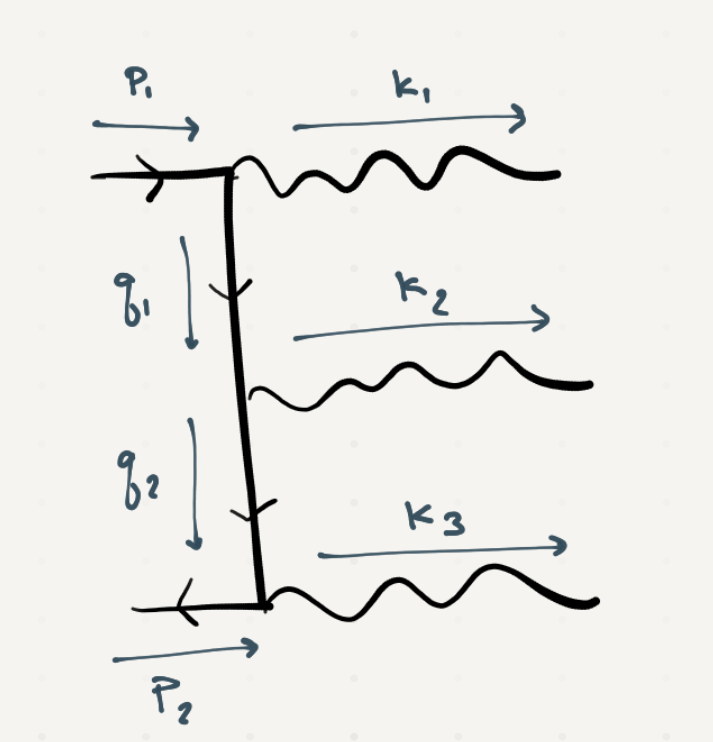
\includegraphics[width=.3\textwidth]{HW2a.png}
\end{center}
Using the conservation of four-momentum at each vertex, show that the total four-momentum is conserved. That is, prove:
\begin{align}
	(p_1 + p_2)^\mu = (k_1 + k_2 + k_3)^\mu \ .
\end{align}
\textsc{Hint:} Start by writing the conservation of four-momentum at each vertex. Those are three equations
%\footnote{...well, 3$\times$4 equations if you count each component separately...} 
with unspecified $q_1^\mu$ and $q_2^\mu$. Use two equations to determine what these virtual momenta are, then plug them into the last equation to prove the above relation.

\section{\texorpdfstring{QED+$\mu$}{QED plus Muon}}

Here are the Feynman rules for ``QED+$\mu$,'' a theory of electrons, photons, and a second type of matter: muons, denoted $\mu$. 
\begin{center}
	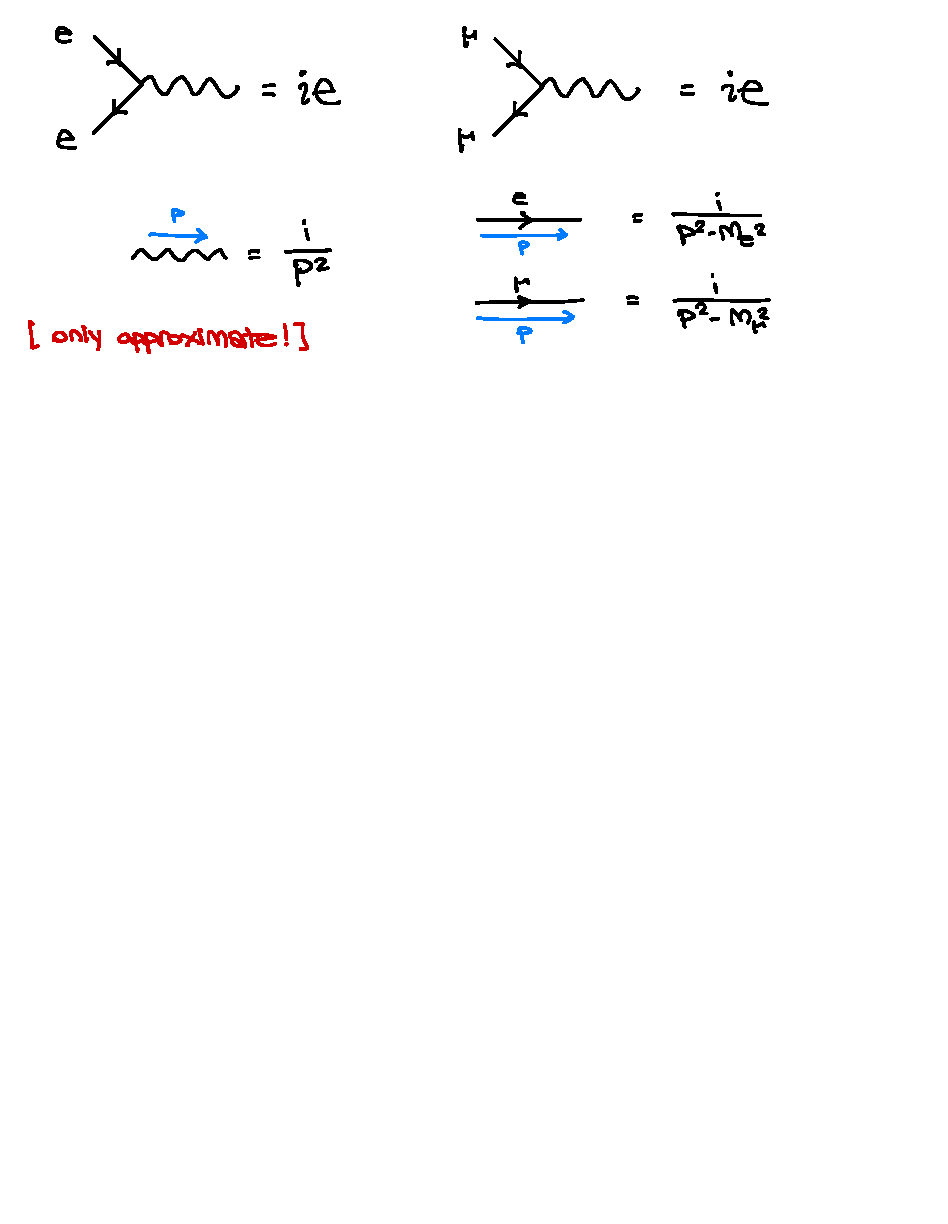
\includegraphics[width=.7\textwidth]{figures/HW4a_muon.pdf}
\end{center}
Muons have the same charge as electrons and so the strength of their vertex with the photon is exactly the same. What are the conserved charges in this theory?

\textsc{Hint:} as you can guess, electric charge is conserved. However, there's a bit more to it than that. For example, $\mu^- \to e^- \gamma$ conserves electric charge. When the muon mass $m_\mu$ is larger than the photon mass, then $\mu^-\to e^-\gamma$ is even kinematically allowed. However, this process cannot happen dynamically in the theory QED+$\mu$. 

\textsc{Comment:} Professor Tanedo's early Ph.D research focused on this process for theories with extra dimensions.\footnote{\url{https://arxiv.org/abs/1004.2037}}


\end{document}